\section{Introduction}
\label{sec:intro}

\begin{comment}
-- OUTLINE
a. Define counterfactual. counterfactuals are how we understand stuff (cite psychology papers) and run decent experiments. Counterfactuals are hard in the real world (cite pearl), but easy if we're analyzing a model
b. Current counterfactuals in NLP: useful for training and eval (contrast sets), but done by hand. Too much work, relies on creativity, may miss stuff. For explanations: adversarial examples, or simple word substitutions.
c. We formalize the task of counterfactual generation: given x, produce \xp, and then rank according to the task. We train a model to do this (some detail).
d. we apply the model to training, eval, explanations. summary of results. Important: compare to counterfactuals created by hand, this is better and faster
\end{comment}

Counterfactual reasoning --- mentally simulating what \emph{would have happened} if conditions were different --- is a common tool for making causality assessments~\cite{kahneman}, which in turn are crucial for explanation~\cite{miller}, evaluation, and model training. For example, in Figure~\ref{fig:teaser}, $x=$ \exinline{It is great for kids} is perturbed into $[\xp_1, \xp_2, ...]$ in such a way that the changes from $x$ to $\xp_i$ brings various insights by simulating what would have happened to if $x$ was different.

Applications of counterfactual reasoning to Natural Language Processing (NLP) generally specify what the $x \rightarrow \xp$ relationship is, and then ask humans to manually create counterfactuals $\xp$, or perturbation functions that generate $\xp$.
For example, \citet{gardner2020contrast} and \citet{kaushik2019learning} ask humans to create counterfactuals $\xp$ that are as close to $x$ as possible \emph{but have a different groundtruth label}, which are used to improve training and evaluation. 
Similarly, \citet{wu2019errudite} and \citet{checklist:acl20} ask humans to create counterfactual-generating functions such as ``remove negation'' or ``add irrelevant information'' in order to verify or test specific model behaviors (\eg whether models handle negation appropriately).
These are costly to generate, and may miss important patterns due to their reliance on human creativity (\eg humans may cover \swap{great}{not great}, but can easily miss \swap{kids}{no one}).
Another application is adversarial example generation, where the relationship between $x$ and $\xp$ is difference in model prediction \emph{and} semantic equivalence~\cite{iyyer2018adversarial, ribeiro2018semantically} --- the later constraining most perturbations to be word replacements or paraphrasing.
In this rare case where counterfactuals can reliably be produced automatically, humans are not able to produce counterfactuals with the desired property as well as automatic methods~\cite{ribeiro2018semantically}, even though they excel at evaluating such counterfactuals.
%TODO: NEed to say something about Li et al 2020 Linguistically-Informed Transformations (LIT): A Method for Automatically Generating Contrast Sets, maybe something about word substitution

\begin{figure}[t]
\centering
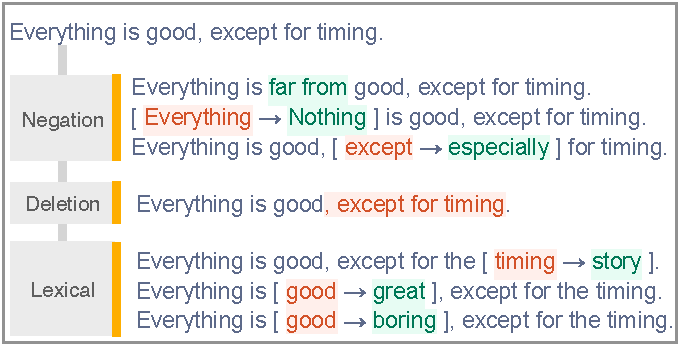
\includegraphics[trim={0 17cm 26cm 0cm},clip, width=1\columnwidth]{figures/teaser}
\vspace{-15pt}
\caption{
The process of \sysname on a sentiment analysis instance.
Given an original $x$ (A), we first generate (B) a large number of $\xp$-s, which are then (C) sorted and selected for different downstream use cases.}
\vspace{-15pt}
\label{fig:teaser}
\end{figure} 
 

In this work, we formalize the task of \emph{automatic counterfactual generation}, where given an input $x$, the goal is to produce a set of counterfactuals $[\xp_1, \xp_2, ...]$ with reasonable relationships $x \rightarrow \xp_i$. 
We frame the task as text generation, and finetune GPT-2 \cite{radford2019language} on combined datasets that have $(x, \xp)$ pairs, such that it can generate general purpose counterfactuals. 
We also allow for targeted counterfactuals, by specifying where the perturbation occurs in the sentence \cite{donahue2020enabling} and using control codes such as \ctrltag{negation}, \ctrltag{delete}, or \ctrltag{lexical} (Figure~\ref{fig:teaser}B). 
The produced set of counterfactuals is then ranked or filtered (Figure~\ref{fig:teaser}C), depending on the applications of interest.
%TODO: need a name here

Through experiments on different classification tasks (Sentiment Analysis, Natural Language Inference, and Duplicate Question Detection), we demonstrate the usefulness of \sysname in three scenarios that require counterfactual reasoning: training, evaluation, and explanation. 
For training and evaluation, we observe that asking humans to evaluate counterfactuals is enough to produce high-quality contrast sets~\cite{gardner2020contrast}, and training data that results in higher generalization accuracy (measured by out-of-domain datasets, challenge sets, contrast sets, and CheckLists~\cite{checklist:acl20}).
Compared to the more difficult task of \emph{creating} one counterfactual, the evaluation process is at least 40\% more effective in terms of creation time, even after aggressive filtering.
% (30 seconds for validating three $\xp$ around one $x$) 

We also use \sysname to produce \emph{black-box counterfactual explanations}. 
Research from the social sciences indicates that counterfactual contrast cases are more intuitive as explanations \cite{miller}.
We prioritize counterfactuals with \emph{abnormal} model behaviors, \ie the actual changes in prediction do not match the expectation (measured by sentence similarity or perturbed feature weights.)
In a model simulation user study, we observe that these explanations can complement popular feature attribution methods such as SHAP~\cite{NIPS2017_7062} by highlighting their missed blind spots: 
After SHAP weights and interacting with the model, NLP experts simulate \tofix{5\%} and \tofix{25\%} more abnormal ones incorrectly, compared to human-generated or random counterfactuals.